%% LyX 2.0.6 created this file.  For more info, see http://www.lyx.org/.
%% Do not edit unless you really know what you are doing.
\documentclass[english]{report}
\usepackage{ccfonts}
\usepackage{avant}
\renewcommand{\ttdefault}{cmtt}
\renewcommand{\familydefault}{\rmdefault}
\usepackage[T1]{fontenc}
\usepackage[utf8]{luainputenc}
\setcounter{secnumdepth}{3}
\setcounter{tocdepth}{3}
\usepackage{amsmath}
\usepackage{amssymb}
\usepackage{graphicx}

\makeatletter
%%%%%%%%%%%%%%%%%%%%%%%%%%%%%% User specified LaTeX commands.
\usepackage{braket}

\makeatother

\usepackage{babel}
\begin{document}

\title{The Ion Trap Architecture}


\title{Atul Singh Arora}
\maketitle
\begin{abstract}
In my course of study so far, I've realized that there're atleast
two good ways of studying new material. The first is to read the content
as a hint (pretend like you're in the past and its coming from the
future) to yourself for developing a new subject from scratch. Your
mind won't question everything and automatically try to get the point.
The other is to understand every single word of the material so you've
mastered it when you're through. The first chapter and second (last)
chapter reflect the corresponding strategies.
\end{abstract}
\tableofcontents{}

\listoffigures



\chapter{Oversimplified overview}


\section{Prerequisites for the chapter}

Can read and take being made fun of occasionally in good spirit. Also
it'll help if you have some rough idea about what Qubits etc. really
are and their use in the context of information processing.


\section{The meat (or vegetable if you prefer)}

If you've read Griffiths with any love, you would know that Earnshaw's
thoerem prohibits creation of a minima using electrostatic potential.
(now don't ask which Griffiths) Thus you can't trap ions conventionally.
\begin{enumerate}
\item Confining the ions

\begin{enumerate}
\item Production of ions: Heating calcium in high vaccuum | fire high speed
electrons | some resulting ions fall inside the trap and get stuck
\item Trap structure: \\
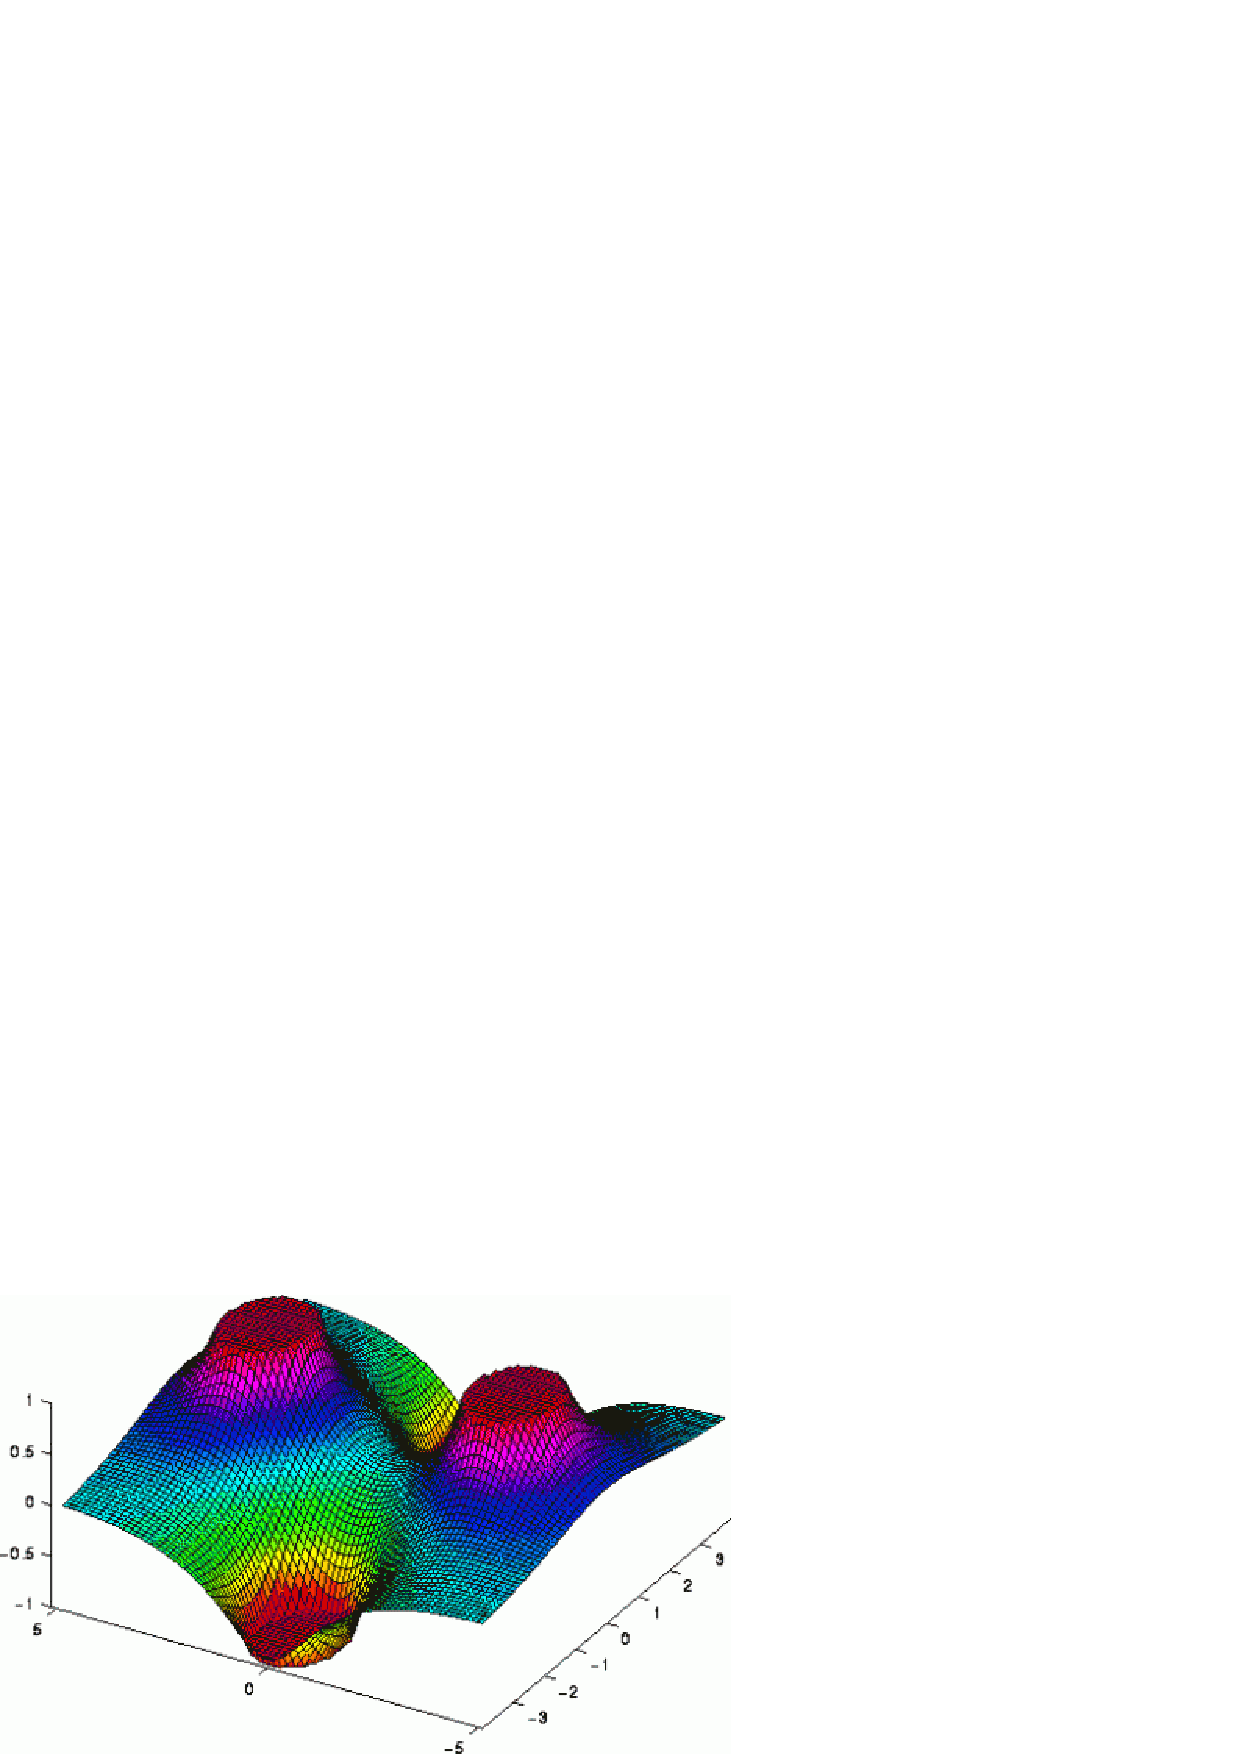
\includegraphics{potential}\\
The idea is simple. Since you can't create a potential minima anywhere
inside the boundary, you can't trap an ion. But you see the saddle
point. You change the potential rapidly so that the `U' minima oscillates
between being along the X and Y axis (say). This way, on an average,
the saddle point sees zero average potential. If the ion were anywhere
other than this point, it'll experiences oscillating forces. This
effectively results in confinement of the atom. Q1. How does an oscillating
force ensure confinement? Q2. What frequencies are most effective
and why? Q3. How do you know only 1 ion is trapped? \\
The next immediate question is what restricts the ion in the Z axis.
Well, we just pin the ion using a positive potential (by putting two
electrodes along the said axis.)
\end{enumerate}
\item Controlling the trapped ions

\begin{enumerate}
\item Let's say that it is obvious we need the kinetic energy of the ions
to be much smaller than that it picks up upon interaction with a laser
(or upon emitting a single photon). This number turns up to be about
32 K Hertz (Energy/Plank's constant). The corresponding temperature
to have thermal energy lower than this, turns out to be a few micro
kelvins!\\
This is a serious challenge.
\item How do you circumvent this? Laser cooling. Oximoron you might say
but the following little thought is illuminating. If you hit an atom
with light with opposite momentum, the atom slows down as the light
is bounced back. So if you could get the ions to absorb light preferentially
going opposite in direction to their momentum, you've found a groundbreaking
method of cooling!\\
And yes, somebody thought of that too. You use something you're already
familiar with, resonance and doppler.

\begin{enumerate}
\item Resonance: This is the (in)famous phenomenon where an innocent and
mild vibration can cause an otherwise stable system to have almost
devastating effects, given the frequency is just right. A similar
effect is observed with atoms and with remarkable sensitivity to the
precision of the frequency. Light is absorbed by the atom only when
the frequency is just right.
\item Doppler: This is as you're well aware, the principle behind the sound
effect you get when a car zooms past. We exploit this and set the
frequency of the laser just below the resonant frequency. This does
it then.\\
NOTE: This is not at all this simple. Q1. If the photon is absorbed,
it must be emitted giving the atom a push again! Whats wrong? Q2.
What about line broadening etc.?
\end{enumerate}
\end{enumerate}
\item Lets get Quantum Computing!

\begin{enumerate}
\item Ions as Qbits: Every ion is one qubit. (In these experiments, we deal
with 3-4 Qbits.) To process information on these qubits, we need to
be able to 

\begin{enumerate}
\item Initialize each qubit individually: This is done by shining light
on it since they're physically separated enough and as the laser light
can be focussed to distances much smaller than that between adjacent
ions.
\item Perform C-NOT between any pair of Qubits (either can be the control/target)
\end{enumerate}
\item Ions as tiny magnets: The ion can be thought of as a tiny magnet.
We can code point up to be state zero and pointing down to be state
one. So far it is the same as classical information storage. However,
quantum mechanically, the magnet can `point in other directions'.
This is perhaps best understood as some sort of angle the magnet is
at with the z-axis (the direction of an external magnetic field).
However this is not a conventional angle. When you make a measurement,
you'll get state zero or one with probabilities proportional to the
projection along the relavent axis. (Its very handwaving but gets
the idea across. Do not extend this picture too much without proper
formalism) This is then as though the atom is in a superposition of
zero and one states and you get one of them upon measurement.\\
This is exploited for information processing. How we probe the ion
(qubit) is by using light. Its interaction with the ion can be understood
as

\begin{enumerate}
\item Classically; it changes the orientation of magnet as light has (is?)
electromagnetic fields. The magnet has again, a frequency dependent
response and the twist magnitude can be controlled by the duration
of the pulse.
\item Quantum(ly?); the laser mixes the zero and one states. The frequency
and duration can be used to calculated precisely the mix created,
enabling us to create the desired superpositions.
\end{enumerate}
\item The computer; ion string: Lets quickly review what C-NOT does. You
flip the target iff the control is one. So, in our setup, the problem
is to flip the state of ion B, iff ion A is in (say) state one (magnet
pointing down). Note that we can't quite use the magnetic field of
the ions themselves for, one they're too small and two, ion A and
B may not be adjacent. Seems like a deal breaker. But these people
(the real scientists) are clever.\\
It goes something like this

\begin{enumerate}
\item A laser light is shone on ion A such that its absorbed only in state
one.

\begin{enumerate}
\item An ion with magnet down (state one), resonates at a slightly different
compared to one with magnet up. Thus it is possible.
\item The ion is given a little more energy (higher frequency). Why, well
cause the ions are able to rattle to and fro their position in the
trap. However this is in a plane perpendicular to the line of ions
(the string). A vibration in this plane is transmitted to all the
ions, because of their charge, viz. interaction by coulombic forces.
Now as we are dealing with single ions, it so happens that this whole
string vibration is also quantized! Thus we give this exact energy
extra in the laser beam.
\end{enumerate}
\item With the entire string vibrating, conditioned by if ion A is in state
one, we shine a light on ion B with a little less energy. If the string
is already vibrating, this would be sufficient to interact with B.
This causes ion B to flip its state iff ion A is in state one.
\item Finally, a beam of light is shone on ion A again to kill the vibration
of the string.
\end{enumerate}
\end{enumerate}
\end{enumerate}
And that's how its done! Ladies and Gentlemen, we have the ion trap
quantum computer architecture. \\
Ofcourse, we've made far too many assumptions but the rough idea should
be clear now. In the following (last) chapter, we address some of
the remarks/questions you might have (such as what the hell, how do
you do that etc.)


\chapter{Prologue; the trap}


\section{Minimum Requirements (for the computer and the reader)}

It has been assumed that the reader has a basic knowledge of quantum
mechanics (Dirac's formulation preferably) and also understands qubits
and their role in information processing. The following is intended
to briefly review some concepts that'll be used and to comment on
some aspects specific to the architecture.

It can be shown that to produce arbitrary unitary transformations
of the state of a set of qubits, it is sufficent to be able to produce
arbitrary rotations in the Hilbert space of any individual qubit and
to be able to carry out the controlled-rotation operation.

Although conventionally we use C NOTs instead of C ROTs, the latter
is more important for it is easier to implement physically and thus
the changed generalization.

However, a further simplification made can be made as follows. Instead
of seeking CROT between any pair of qubits directly, it is sufficient
to have one special qubit which can undergo CROT with any of the other.
This special qubit is refered to as a 'bus' and can be used to carry
information around using another gate called SWAP (does what it says,
swaps the qubits). Although this can be decomposed into the aforesaid
gates, in practice, this can be directly implemented physically. The
major disadvantage of the bus method is that parallel operations aren't
possible.

Accepting the limitations and proceeding with the 'bus' idea, we have
the following minimum requirements of our quantum processor.
\begin{enumerate}
\item Arbitrary rotations of any single qubit
\item CROT between the bus and any other qubit (note, the other way round
is not required, viz. the control is bit is the bus)
\item SWAP between the bus and any other qubit
\end{enumerate}
It will be shown in the following section how all of these can be
achieved on the ion trap architecture. Other than this ofcourse, we
must be able to make measurements also.

Further, it is worthwhile to remark that a processor with a few qubits
may be built using a single particle with sufficient degrees of freedom.
The ion trap approach however is more sensible in realizing an interesting
enough quantum computer, with say a hundred qubits.


\section{Setup, the trap}


\subsection{Introduction}

We discuss here an ion trap with a line of N trapped ions. Each ion
has two stable and two metastable states (such as hyperfine or two
zeeman levels). There's a setup to point laser beams to interact with
any of the N ions. Each ion constitutes one qubit; the two internal
energy eigenkets of the ion. There's also the bus qubit discussed
in the previous section. The vibrational motion of the whole string
of ions constitutes this qubit. This motion must be quantized for
it to be usable as a qubit. This thus requires cooling the ion string
well below the `quantum limit', defined with respect to the axial
vibrational frequency,
\[
k_{B}T\ll\hbar\omega_{z}
\]


This happens to be one of the most challenging parts of the experimental
setup, after making the trap and catching the ions. (Subtleties related
to the ``Lambe-Dicke'' regime haven't been discussed) Further, in
brief, there're two known traps, the Paul (rf) and the Penning (Magnetic)
and it so turns out that the former allows for tighter confinement
(useful for cooling) and allows for magnetic fields to be used for
other useful purposes such as splitting into zeeman levels. Further,
tighter trapping leads to faster `switching time' for quantum gates
such as CROT to be discussed in the next section.


\subsection{Modeling the motion}

The N trapped ions are modelled as a system of N point charges in
a harmonic potential well of tight radial confinement, viz. $\omega_{x},\omega_{y}\gg\omega_{z}$.
Obviously, the parameters $\{\omega_{i}\}$ will be determined by
the electrode geometry and potentials, which will not be discussed
in this report. The corresponding hamiltonian is

\[
H=\sum_{i=1}^{N}\frac{1}{2}M\left(\omega_{x}^{2}X_{i}^{2}+\omega_{x}^{2}Y_{i}^{2}+\omega_{x}^{2}Z_{i}^{2}+\frac{\mathbf{P}_{i}^{2}}{M^{2}}\right)+\sum_{i=1}^{N}\sum_{j>i}\frac{e^{2}}{4\pi\epsilon_{0}|\mathbf{R}_{i}-\mathbf{R}_{j}|}
\]
 where the position and momentum are operators. Assertion: at low
temperatures, for tight radial confinement, the ions all lie along
the z-axis. Consequently it is reasonable to assume $|R_{i}-R_{j}|\approx|Z_{i}-Z_{j}|$
which allows for the radial and axial motion to be separated. Considering
the axial motion, we first find a relevant length scale, say 
\[
z_{s}=\left(\frac{e^{2}}{4\pi\epsilon_{0}M\omega_{z}^{2}}\right)^{1/3}\approx10-100\,\mu m
\]
which is of the order of separation between the ions. Solving the
equation classically, one obtains the equilibrium positions of the
ions. As is expected, for larger N, the outer ions tend to push the
inner ions closer. Consequently, the spacing between the ions depends
upon N. However, it is not so obvious that the two normal modes of
oscillation about these equilibrium positions are independent of N
(for small oscillations that is). Besides, even higher harmonics are
nearly independent of N. The frequencies of the two normal modes are
$\omega_{z}$ and $\sqrt{3}\omega_{z}$ (the list goes $\{1,\sqrt{3},\,\sqrt{29/5},\,3.051,\,3.671,\,4.272,\,4.865\dots\}$
times $\omega_{z}$). In the lowest of mode of oscillation all the
ions move to and fro together. This mode thus corresponds to the harmonic
motion of the centre of mass of the ion string. Since the frequencies
of the higher harmonics are so different from that of the ground normal
mode, it can be excited selectively, without exciting the other modes. 

So far everything was classical. In cranking things up to the quantum
level, we simply treat the centre of mass coordinate $z_{cm}$ as
a harmonic oscillator. We assert that the classically determined ground
state excitation frequency $\omega_{z}$ continues to be valid even
though the ion wave functions now overlap; they delicately cancel
upon calculation of the centre of mass motion. Accepting this assertion,
we proceed by noting that the harmonic oscillator has $NM$ mass and
frequncy $\omega_{z}$. Thus the energy eigenfunctions are given as
\[
\psi_{n}(z_{cm})=\left(\frac{NM\omega_{z}}{\pi\hbar2^{2n}(n!)^{2}}\right)^{1/4}H_{n}\left(z_{cm}\sqrt{NM\omega_{z}/\hbar}\right)e^{-NM\omega_{z}z_{cm}^{2}/2\hbar}
\]
This gives us the extent of spatial spread of the ground state probability
distribution, which is given by its standard deviation, 
\[
\Delta z_{cm}=\sqrt{\hbar/2NM\omega_{z}}
\]
We certainly don't want our inter-ion distance to be comparable to
$\Delta z_{cm}$, else addressing each ion individually with a laser
beam would become unnecessarily hard, if not impossible. Thus we require
$\Delta z_{cm}\ll\Delta z_{min}$. A numerical solution yields 
\[
\Delta z_{min}\approx2.0z_{s}N^{-0.57}
\]
where $z_{s}$ is the length we found in the beginning (this formula
remains valid till $N\approx1000$). Imposing the inequality we get
\[
\frac{\omega_{z}}{M}\ll\frac{31N^{1.86}}{\hbar^{3}}\left(\frac{e^{2}}{4\pi\epsilon_{0}}\right)^{2}\approx2.4\times10^{21}N^{1.86}\,\text{Hz/u}
\]
where u is the atomic mass unit ($1.66057\times10^{-27}$ kg). The
parameters here are the frequency which we said depends on the geometry
and potentials of the electrodes. The mass of the atom is also somewhat
in our control (depends on which we choose, but there're other factors
influencing that also). However, in practice, this condition is found
to be easily satisfied. $\omega_{z}$ is no more than a GHz, while
$M$ ranges from 9 to 200 u. It's thus accurate to image the ions
as sitting on a line, with their small wavepacket centred at their
classical equilibrium location, with essentially no overlap with others.
It must be stated that this condition alone doesn't guarantee that
the separation is enough to allow unique addressing of the ions by
laser beams.


\section{Matrix: From paper to our loyal ions}


\subsection{The states we make}

First things first. What are the states we're looking at and how long
will excited states last. Lets answer them. There are two kinds of
states. 
\begin{enumerate}
\item The first are internal energy eigenstates of the ion. (refer to the
figure)

\begin{enumerate}
\item We write these states as $\ket{F_{1},M_{1}},\,\ket{F_{2},M_{2}}$
and $\ket{F_{aux},M_{aux}}$ 
\item They are separated by $\omega_{0}$ and $\omega_{aux}$ as shown.
\end{enumerate}
\item The other are the excitations of the centre of mass motion.

\begin{enumerate}
\item The eigenkets of the vibrational motion are written as $\ket{\{n_{i}\}}$
where $n_{i}$ are the excitations of the various modes. 
\item Only the ground state $\ket{0,0,0\dots}$ and the first excited state
$\ket{1,0,0\dots}$ are invoked for the operations
\item This state is loosely called the phonon (used here as the bus bit)
\end{enumerate}
\end{enumerate}
So the states we'll be finally working with, will be the following
tensor products

\[
\begin{aligned}\ket{0,0}\equiv\ket{F_{1},M_{1}}\otimes\ket{0,0,0\dots}\\
\ket{0,1}\equiv\ket{F_{1},M_{1}}\otimes\ket{1,0,0\dots}\\
\ket{1,0}\equiv\ket{F_{2},M_{2}}\otimes\ket{0,0,0\dots}\\
\ket{0,1}\equiv\ket{F_{2},M_{2}}\otimes\ket{1,0,0\dots}
\end{aligned}
\]


That answers the first question. The second is answered by the well
known (but not well understood for me so far) energy time uncertainty
relation, which unlike the unambiguous position momentum uncertainty
arising from the commutation relation, refers to a more general class
of such uncertainty relations (including ones that arise from perturbation
theory). The point is that since all the levels considered here are
low-lying, separated oh so mildly (hyperfine and Zeeman interactions),
that the lifetime of the excited states (against spontaneous emission)
is essentially infinite. 


\subsection{The gates it takes}

We show how to perform the following operations.
\begin{enumerate}
\item \emph{CROT} between any ion's internal state and the phonon bit, where
CROT is given by\\
\[
U_{\text{CROT}}\equiv\left[\begin{array}{cccc}
1\\
 & 1\\
 &  & 1\\
 &  &  & -1
\end{array}\right]
\]
in the computational basis, $\ket{00},\ket{01},\ket{10},\ket{11}$.
So in essence, if the internal state is zero, then you do nothing.
Else you apply $\sigma_{z}$ to the phonon.
\item Carry out \emph{arbitrary rotations} in the ion's internal state,
viz. be able to apply \\
\[
e^{-i\theta.\sigma/2}=\left[\begin{array}{cc}
cos(\theta/2) & -e^{-i\phi}sin(\theta/2)\\
e^{i\phi}cos(\theta/2) & cos(\theta/2)
\end{array}\right]
\]

\item Perform a \emph{swap} between any ion and the bus (phonon) bit. The
matrix is obviously\\
\[
U_{\text{SWAP}}\equiv\left[\begin{array}{cccc}
1\\
 & 0 & 1\\
 & 1 & 0\\
 &  &  & 1
\end{array}\right]
\]

\end{enumerate}
It is known that these three operations together can be used to carry
out arbitrary transformations to the qubits stored. 


\subsubsection*{CROT}

Remember there were these $\ket{F_{aux},M_{aux}}$ eigenstates of
the ion which we didn't use in the definition of the computational
basis $\ket{0,1},\ket{0,1}$ etc. We now define 
\[
\ket{aux,i}=\ket{F_{aux},M_{aux}}\otimes\ket{i,0,0,0\dots}
\]
where $i\in\{0,1\}$. These states are available to us as kind of
shelves. These help us make state-dependent transformations (such
as controlled rotations). 

A look at the figure shows that if a radiation of frequency $\omega_{aux}+\omega_{z}$
is applied, then only transitions between $\ket{1,1}$ and $\ket{aux,0}$
will occur (assuming states in unwanted levels are unoccupied). \\


\emph{Claim: If a $2\pi$ pulse (of the said frequency) is applied,
then the state $\ket{1,1}$ is rotated by $2\pi$ radians. }

This is precisely what was required. If the state is $\ket{1,1}$
its sign is flipped. (Note: Don't confuse the state of the computational
basis with that of the auxilary state, which is in a zero phonon state)\\


\emph{Claim: A $2\pi$ pulse of frequency $\omega_{z}-(\omega_{0}-\omega_{aux})$
produces a control rotation corresponding to} 
\[
U_{\text{C\ensuremath{\rightharpoondown}ROT}}\equiv\left[\begin{array}{cccc}
1\\
 & -1\\
 &  & 1\\
 &  &  & 1
\end{array}\right]
\]


Justification: This should be obvious from the previous discussion
and the diagram. Effectively then, $U_{\text{C\ensuremath{\rightharpoondown}ROT}}$
rotates the second qubit if the first is in state zero rather than
one.


\subsubsection*{Arbitrary Internal State Rotations}

To rotate an ion's internal state without affecting the phonon (centre
of mass motion), a pulse of frequency, without surprise, $\omega_{0}$
is applied. (This part is not too clear) \\


\emph{Claim: If such a radiation has a phase $\phi$ wrt some defined
origin of phase, and duration sufficient to make a $p\pi$ pulse,
then the effect in the computational basis is
\[
V^{p}(\phi)\equiv\left[\begin{array}{cc}
cos(p\pi/2) & -e^{-i\phi}sin(p\pi/2)\\
-e^{i\phi}cos(p\pi/2) & cos(p\pi/2)
\end{array}\right]\otimes\left[\begin{array}{cc}
1 & 0\\
0 & 1
\end{array}\right]
\]
}To apply such rotations successfully, it is required that experimentally,
the phase is controlled at the position of the ion (and not just some
other physical location, like a stable reference cavity). In this
regard therefore it is much easier if the computational basis of the
system are separated by radio frequencies and not optical frequencies.\\


\emph{Claim 2: In order to have the right phase experimentally, one
needn't worry about the continuous precession with $\omega_{0}$ caused
by the internal Hamiltonian of each ion}\\


\emph{Claim 3: However problems arise when different ions have different
frequencies due to the residual electric and magnetic fields in the
apparatus, although such problems are solvable.}\\



\subsubsection*{Universalization: CNOT detour}

We have already developed enough machinery to implement an XOR (a
reversible XOR is the same as a CNOT) between the bus (phonon) and
some particular ion. To recall, C NOT is defined as
\[
\text{XOR}\equiv\left[\begin{array}{cccc}
1\\
 & 0 & 0 & 1\\
 & 0 & 1 & 0\\
 & 1 & 0 & 0
\end{array}\right]
\]
The matrix is wrong isn't it? No! We are doing a CNOT(bus,ion) as
opposed to CNOT(ion,bus). Here's the sequence that does the trick
\begin{enumerate}
\item A $\pi/2$ pulse with frequency $\omega_{0}$
\[
V^{1/2}(-\pi/2)=\frac{1}{\sqrt{2}}\left[\begin{array}{cc}
1 & 1\\
-1 & 1
\end{array}\right]_{\text{ion}}\otimes\left[\begin{array}{cc}
1 & 0\\
0 & 1
\end{array}\right]_{\text{bus}}
\]

\item CROT
\item Another $\pi/2$ with frequency $\omega_{0}$ and phase $\pi$ wrt
the first, viz $V^{1/2}(\pi/2)$
\end{enumerate}
Q1. How did they come up with this? Whats the rationale behind this?\\


It can be checked that the result is infact XOR(bus,ion) as given
by the matrix above. So by symmetry XOR(ion,bus) should be a similar
sequence with $\omega_{0}$ replaced with $\omega_{z}$ to cause the
vibration (bus) level to get affected independent of the ion. Right?
Nope. Let's understand this. 

The basic issue is that vibrations (the bus) aren't a two level system.
And where does this bite us? Well, recall how in the implementation
of the CROT we assumed that $\ket{aux,1}$ is unoccupied, for if it
were, then upon flashing $\omega_{aux}+\omega_{z}$ it would merrily
couple to $\ket{1,2}$ which is, surprise surprise, outside our computation
Hilber space!


\subsubsection*{SWAP}

Well this is by far the easiest to implement. Just consider the frequncy
$\omega_{0}-\omega_{z}$ and look at the transitions diagram. The
only possible transition is between $\ket{01}$ and $\ket{10}$ (assuming
ofcourse there's no population in the $\ket{11},\,\ket{02}$ states
etc.). So then that does it! We have swapped successfully between
the bus and any one of the ions.\\


And that completes the gates part.


\subsection{How to see without mistakes}

To complete the operation of the processor, we must be able to make
measurements. This is achieved with high accuracy, using what is known
as `electron shelving' or `quantum jumps' technique. This results
in whether the ion is in the $\ket{F_{1}M_{1}}$ or $\ket{F_{2}M_{2}}$.
This is achieved by illuminating the ion with a radiation resonant
with a transition from $\ket{F_{1}M_{1}}$ to some high-lying level,
whose line-width is sufficiently small so that transitions from $\ket{F_{2}M_{2}}$
aren't excited (else what's the point eigh?). Now if the flourescence
is produced, the ion state has collapsed to $\ket{F_{1}M_{1}}$; if
its not produced, then you know it is in $\ket{F_{2}M_{2}}$. Note
that you can't readout the bus directly, but since you can swap, it's
not an issue now is it?

So in effect, do you realize what you've done? If this doesn't blow
your mind, then you have no feelings!


\section{Essential and missing}

There are some essential topics which haven't been discussed here
but have been mentioned here.
\begin{enumerate}
\item Cooling
\item Design of the ion trap itself
\item Candidate ions
\item Errors and limitations\end{enumerate}
\begin{thebibliography}{1}
\bibitem{key-1}https://www2.physics.ox.ac.uk/research/ion-trap-quantum-computing-group/intro-to-ion-trap-qc

\bibitem{key-2}http://xxx.soton.ac.uk/abs/quant-ph/9608011

\bibitem{key-3}\end{thebibliography}

\end{document}
